%!TEX root = thesis.tex

\chapter{Body Part Detection}
\label{ch:bodyparts}

To perform hand pose estimation of a person in a image his or her hands need to be localized in the image first. Since hands can have different shapes, different orientations, specific color profiles and shapes per person this is a very difficult task. One way to localize the hands is by searching for skin like colors in an image given that this color profile is known. A generic skin model has been build for this purpose\cite{Jones1999}, but using these values for searching in a image is quite sensitive for error. Skin color can vary dramatically because of lightning conditions but also the cameras properties can color a image. It would be much better to have a method for obtaining the skin color of the hands from a image itself. This can be done by detecting the subjects face in an image.

\section{Building a skin model}
\label{sec:skinmodel}

\subsection*{Face detection \- Haar classifier}
Finding faces in a image is a rather well solved problem. Faces are easy to detect, since it has easy to detect features like eyes, eyebrows, a mouth and a nose. When comparing different faces, these features are \- with a small variation \- on the same distance and orientation. Also people don't tilt their head often, or not more than a couple degrees. Face detection can be done in a fast and robust way using a haar classifier, a boosted rejection cascade that is trained with Haar\-like wavelet\cite{Lienhart2002}. This is a method for detecting faces that doesn't rely on color information. Using a haar classifier to search for a face and obtain a skin color profile has been done before with the yab color space \cite{Stenger2006}, but in this case the HSV color space is used.


\subsection*{Color space conversion}
Usually pixel values of a image are stored in the Red, Green Blue (RGB) format. Advantages can be gained by converting this color space into an other so, for example thresholding on one or more channels or even leaving one channel out gets a different meaning. One particular color space that is interesting for this application is the Hue Saturation Value (HSV) color space. HSV space separates out Hue (color) from Saturation (how concentrated the color is) and from Value (brightness). When a subject is lighted by a light source with uniform hue distribution, the light doesn't change the hue or saturation of the subject. The only thing that will change is the intensity, which is changing because of the light source's intensity, distance or (self casted) shadow. Since we want to extract hand pixels independent of the lightening intensity, we can ignore this channel and only use the hue and saturation.

As many things in computer vision in theory this should work, but in practice it doesn't or not perfect. A light source never has a uniform distribution and \emph{will} color the subject. But in our case that doesn't matter, since all skin pixels in the image will have the same shift in the hue spectrum.

The RGB color space is transformed into the HSV color space using the following equations:
\begin{eqnarray*}
  V & \leftarrow & \max(R,G,B) \\
  S & \leftarrow & \left\{
  \begin{array}{l l}
    \frac{V-\min(R, G, B)}{V} & \quad \text{if $V \neq 0$} \\
    0 						  & \quad \text{otherwise} \\
  \end{array} \right.\\
  H & \leftarrow & \left\{
  \begin{array}{l l}
    \frac{60(G - B)}{S}     & \quad \text{if $V = R$} \\
    \frac{120 + 60(B-R)}{S} & \quad \text{if $V = G$} \\
    \frac{240 + 60(R-G)}{S} & \quad \text{if V = B} \\
  \end{array} \right.\\
\end{eqnarray*}

\begin{figure}[htbp]
	\center
	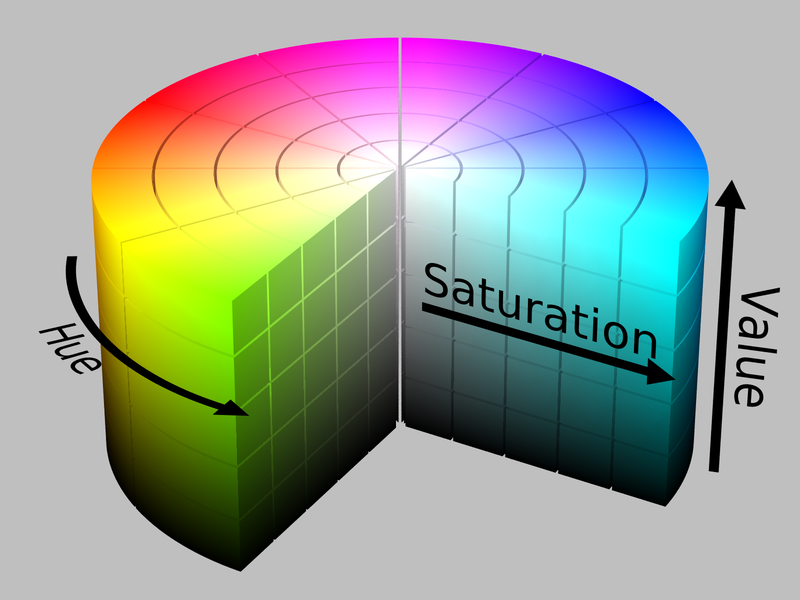
\includegraphics[width=0.4\linewidth]{figures/hsv.png}
	\caption{The Hue, Saturation, Value color space}
	\label{fig:hsv}
\end{figure}

So first the input 3 channel RGB image is transformed into a 3 channel HSV image, where the brightness channel is discarded. From the hue and saturation channel together with the face region we can build a histogram which will represent a statistical skin model.


MISSCHIEN WAT MEER OVER DEZE PAPERS:\cite{Bradski1998}, \cite{Cooper2007}. MAAR IK KAN NIET ECHT IETS VINDEN OVER DAT HUE SAT ECHT ZOVEEL BETER IS DAN ANDERE METHODES. In \cite{Stenger2006} DOEN ZE PRECIES HET ZELFDE MAAR DAN MET YUV.


\subsection*{Skin color histogram}
A histogram is a n-dimensional matrix, where every dimension is divided into bins. In our case there are 2 dimensions, one for hue and one for saturation. A bin corresponds to a range of values for every pixel in the source image. A histogram is constructed by creating an empty matrix. For every pixel in the image the corresponding bin is determined, and the value of the bin is increased by one. The result is a matrix with the count of all the hue and saturation combinations in the source image. There are not really optimal values for the number of bins, around 30 for each is good.\marginpar{WHY}

When all pixels are evaluated, the histogram is normalized - all values are divided by the sum of all bins. This way when all values are added together, the sum will be equal to 1. This makes the histogram independent of the image size, and each value represents a 'skin probability'. Figure\ref{fig:pipe_hist} is a histogram of face pixels.

\subsection*{Back projection}
A back projection is the combination of an image and a histogram. The result is a new single channel image. All pixels in the input image are iterated and the corresponding bins are looked up in the histogram. The pixel in the same position in the new image is replaced with the value from the histogram. If the histogram is a skin color histogram, the resulting image will have high values for pixels that are skin-like pixels, and low values for other pixels. The result of the process can be seen in Figure\ref{fig:pipe_bp}.


\subsection*{Threshold}
To binary label every pixel to be skin color or not, we need to define a way of doing this automatically. The easiest way to accomplish this is by defining a threshold. All pixel values below a certain threshold are replaced with false or 0, all above this threshold will be replaced with true or 1. This results in a binary image with labels for (non) skin pixels. This method introduces one parameter - the threshold for going from the probabilistic domain to the binary domain.


\subsection*{morphological operations}
until now each pixel has been processed independently, and the information in surrounding pixels is ignored. In natural images, very strong gradients (changes from one pixel to the other) are rare. Pixel values close to each other in the image are usually also close to each other in the HSV domain. This is also true for skin like pixels and non skin like pixels. In other words said; if a pixel is for example a skin pixel, then the neighbors are probably also skin pixels and the opposite. To incorporate this implicit information the morphological operations can be used. Also pixels can be noisy, caused by the camera or environment. The pixel value combined (smoothed) with the pixels surrounding the pixel can reduce the influence of this noise. 

There are 2 basic morphological operations which can be used separately or in sequence - the erode operation and the dilate operation which are strongly related. The input for the operations is a binary image and a kernel. A kernel can be any 2D binary matrix, but usually an elliptic shape is used. When performing the erode operation on a input image $A$ with kernel $K$, all false pixels in $A$ are iterated. In every iteration the surrounding pixels of the current iterated pixel are replaced with the false values in $K$, with the center of $K$ as relative point of the current iteration point. The result is that the binary true shapes in $A$ are 'eroded'. This is the same for dilation, but the opposite way. One could also say that in the case of dilation the background, or false pixels are 'eroded'.

A morphologic closing operation of A by B is obtained by the dilation of A by B, followed by erosion of the resulting structure by B. The result of performing this operation is that small holes in the binary image are removed, and edges are smoothed.

\section{Object localization}

\subsection*{Pixel grouping, contour extraction}
To be able to say something useful about groups of pixels, one need to know which pixels belong together. This can be done by clustering. In this case clustering is performed by grouping pixels together to touch horizontally and vertically. This is done with the algorithm described in \cite{Suzuki1985}. This algorithm also constructs a list of pixels that form the border of a group. This list of pixels can be used for many interesting things, like finding the top position of the group in a fast way, or to find out if a unidentified pixel is inside the group. Clustering contour extraction\cite{Suzuki1985}.

From the contours of the group a square region of interest can be defined by calculating the outer borders of the group. This window will be called the hand window.

\subsection*{Blob labeling}
Now we have grouped skin pixels (blobs) we need to know what group of skin pixels is what body part. It is assumed that there is only one person in the image and that the body is covert with clothing except for the head an hands. In a optimal situation this would result in 3 blobs, 2 for the hands and one for the head. For one blob it is already known what body part it is - the face. In the face detection phase we found a face in the image, so the blob containing the center point of the detected phase is the face blob. Usually the left hand is on the left of the head and the right hand on the right side. If there are 3 blobs, and the face is the middle blob, we labeling is done. But unfortunately in practice this isn't always the case. Often there are more or less blobs, because for example an object in the background has skin-like colors or one hand is difficult to detect. Also the order of hands and head can change, a left hand doesn't necessarily need to appear on the left side of a head. In this case some more intelligent decision process. 

First the surface of each blob is calculated and then the blobs are sorted by size. The blob containing the head is removed from the list, since we already know this label. Also very small blobs are removed, because these are probably noise. The removal threshold surface is set to:

\begin{equation}
T = (\frac{h}{20})^2
\end{equation}

All blobs smaller than this value are discarded. 

Assuming the hands or the second biggest skin like objects in the image, the 2 or less biggest blobs are taken from the list and the rest is also discarded. If there is no biggest blob, the labeling is finished - there is only a head in the image. If there is one blob left, the left or right position relative to the head is the hand label. If there are 2 hands, there are 3 possible situations, 1 where the head is in the middle which is already described. If both hands are on the left of the head, the most outer left blob is labeled as left and the other as right. This is visa versa for right.


\subsection*{Blob label stabilization}
A hand doesn't move very fast in an image - usually it will not move from the left side to the right side in one frame. If this is detected this is probably a measurement error caused by noise or pour labeling. In this case the history of previous positions of a blob can be incorporated. This can be done with a Kalman Filter. A Kalman Filter is a easy and fast way of smoothing out the current position with the previous positions. The result will be a more stable estimation of the hand position. A second advantage of the Kalman Filter is the ability to actually predict the position of the hand in the next frame. This can become useful when there is no new hand detected. The hand position can then be estimated with a different method.

For every hand a Kalman filter is initialized. The measurement that need to be smoothed is the hand window. The hand window has a x and y position and a width and hight. Each hand also has a speed in the x and y direction but we don't measure that - we let the kalman filter represent, calculate and use that internally. 

The measurement vector \[ m_k = \left(
\begin{array}{c}
	x_k \\ %measurement.x
	y_k \\ %measurement.y,
	w_k \\ %measurement.width
	h_k \\ %measurement.height
\end{array} \right)\]


The Transition matrix:

\[ A = \left(
\begin{array}{cccccc}
	1 & 0 & 0 & 0 & 1 & 0 \\
	0 & 1 & 0 & 0 & 0 & 1 \\
	0 & 0 & 1 & 0 & 0 & 0 \\
	0 & 0 & 0 & 1 & 0 & 0 \\
	0 & 0 & 0 & 0 & 1 & 0 \\
	0 & 0 & 0 & 0 & 0 & 1 \\
\end{array} \right)\] 

In this matrix  the upleft 2 values represent the combination between the position and the speed.

% setIdentity(kalman.measurementMatrix, Scalar(1));
% setIdentity(kalman.processNoiseCov, Scalar(1));
% setIdentity(kalman.measurementNoiseCov, Scalar(5));
% setIdentity(kalman.errorCovPost, Scalar(3));
% setIdentity(kalman.gain, Scalar(0e-15));
% randu(kalman.statePost, Scalar(1), Scalar(100));



\paragraph{Update}
The kalman filter is then updated:

Innovation or measurement residual 	
$\tilde{\textbf{y}}_k = \textbf{z}_k - \textbf{H}_k\hat{\textbf{x}}_{k|k-1}$

Innovation (or residual) covariance
$\textbf{S}_k = \textbf{H}_k \textbf{P}_{k|k-1} \textbf{H}_k^\text{T} + \textbf{R}_k$

Optimal Kalman gain
$\textbf{K}_k = \textbf{P}_{k|k-1}\textbf{H}_k^\text{T}\textbf{S}_k^{-1}$

Updated (a posteriori) state estimate
$\hat{\textbf{x}}_{k|k} = \hat{\textbf{x}}_{k|k-1} + \textbf{K}_k\tilde{\textbf{y}}_k$

Updated (a posteriori) estimate covariance
$\textbf{P}_{k|k} = (I - \textbf{K}_k \textbf{H}_k) \textbf{P}_{k|k-1}$

\paragraph{Prediction}
And the values are predicted with:

Predicted (a priori) state estimate 	
$\hat{\textbf{x}}_{k|k-1} = \textbf{F}_{k}\hat{\textbf{x}}_{k-1|k-1} + \textbf{B}_{k} \textbf{u}_{k}$

Predicted (a priori) estimate covariance
$\textbf{P}_{k|k-1} = \textbf{F}_{k} \textbf{P}_{k-1|k-1} \textbf{F}_{k}^{\text{T}} + \textbf{Q}_{k}$


\subsection*{template search}
When in a previous frame a hand was detected but in the current frame not any more there is the problem of (self) occlusion. In this case template search is used to track the hand. A cut out image of the hand in the previous frame is used for this template search. Template search is a very simple and quite fast method, as long as the search area is small. A sliding window  with the same size as the cutout image is sliding over a small surrounding area of the location predicted by the kalman filter. The window with the lowest squared sum difference to the previous cutout image is set as the new location. If the original cutout is touching the border of the image or the squared sum difference is to high it is assumed the hand has left the image, and is flagged accordingly. This method works if the shape and size of the hand don't change too much.

\begin{figure}[htbp]
\begin{center}
\subfloat[detected hand]{\label{fig:template_good}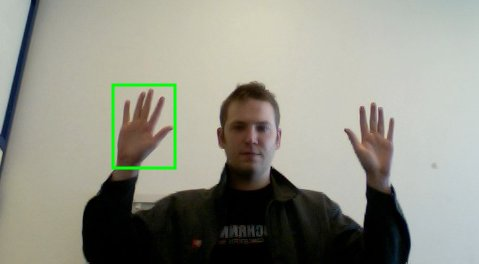
\includegraphics[width=0.45\linewidth]{figures/template/good.jpg}}
\hspace{0.03\linewidth}
\subfloat[result of template search]{\label{fig:template_occlusion}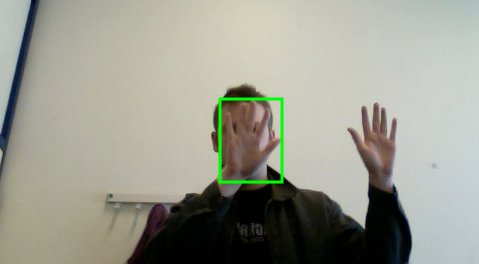
\includegraphics[width=0.45\linewidth]{figures/template/occlusion.jpg}}

\end{center}
\caption{Example of template search}
\label{fig:templatesearch}
\end{figure}

Figure \ref{fig:templatesearch} shows a test setting of a template search. In the left image The left hand was found using the skin model. In the second frame the hand cannot be found, because it is occluding the face and using the skin model approach the hand will be labeled as face. Using a template search the hand can still be tracked.


\section{Discussion}

A parameterless method of going from the probabilistic domain to the binary domain is adaptive thresholding.

The face detection is one of the most expensive operations in the processing chain. Since in a single shot movie usually a face doesn't move fast, a number of frames can be skipped which will free more computational time for other operations.

\begin{figure}[htbp]
\begin{center}
\subfloat[input frame]{\label{fig:pipe_input}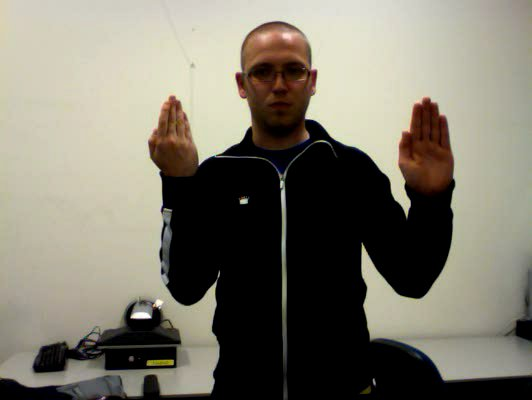
\includegraphics[width=0.3\linewidth]{figures/pipeline/input.jpg}}
\hspace{0.03\linewidth}
\subfloat[hue channel]{\label{fig:hue}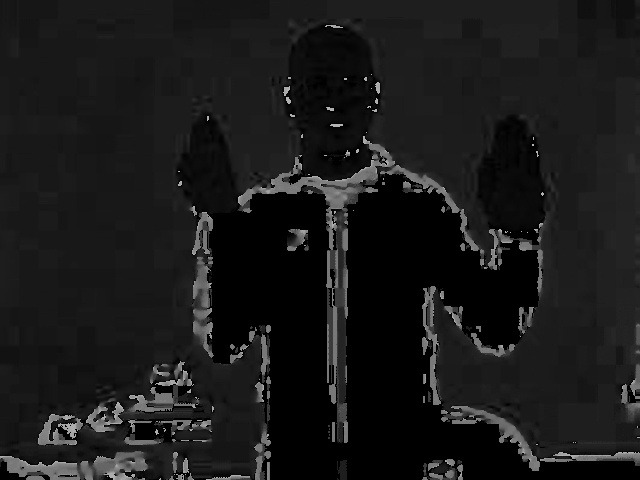
\includegraphics[width=0.3\linewidth]{figures/pipeline/hue.jpg}}
\hspace{0.03\linewidth}
\subfloat[saturation channel]{\label{fig:saturation}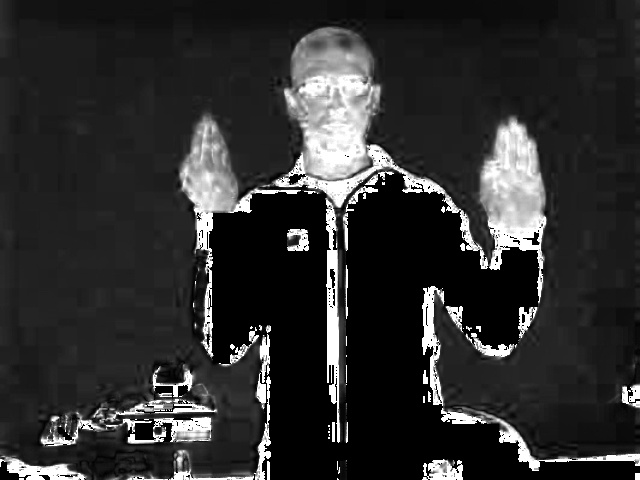
\includegraphics[width=0.3\linewidth]{figures/pipeline/saturation.jpg}}
\hspace{0.03\linewidth}
\subfloat[value channel]{\label{fig:value}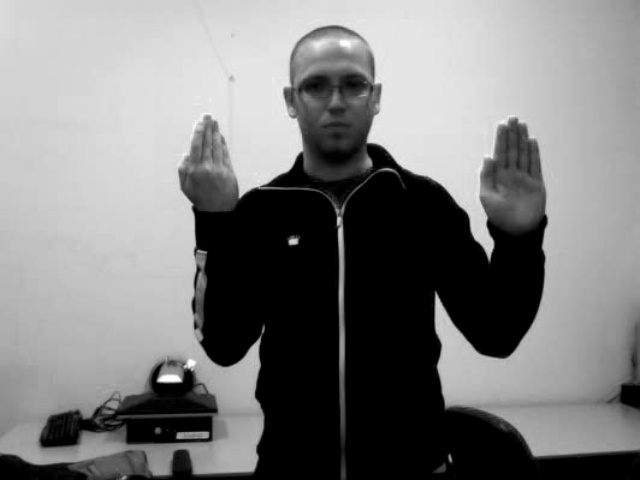
\includegraphics[width=0.3\linewidth]{figures/pipeline/value.jpg}}
\hspace{0.03\linewidth}
\subfloat[face detection]{\label{fig:pipe_detected}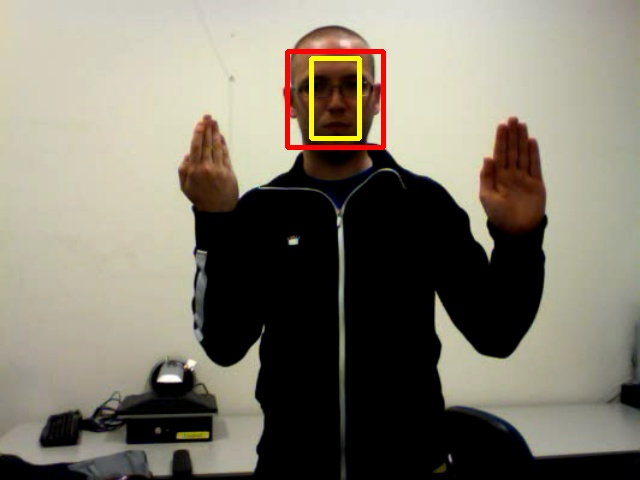
\includegraphics[width=0.3\linewidth]{figures/pipeline/detected.jpg}}
\hspace{0.03\linewidth}
\subfloat[Face color histogram]{\label{fig:pipe_hist}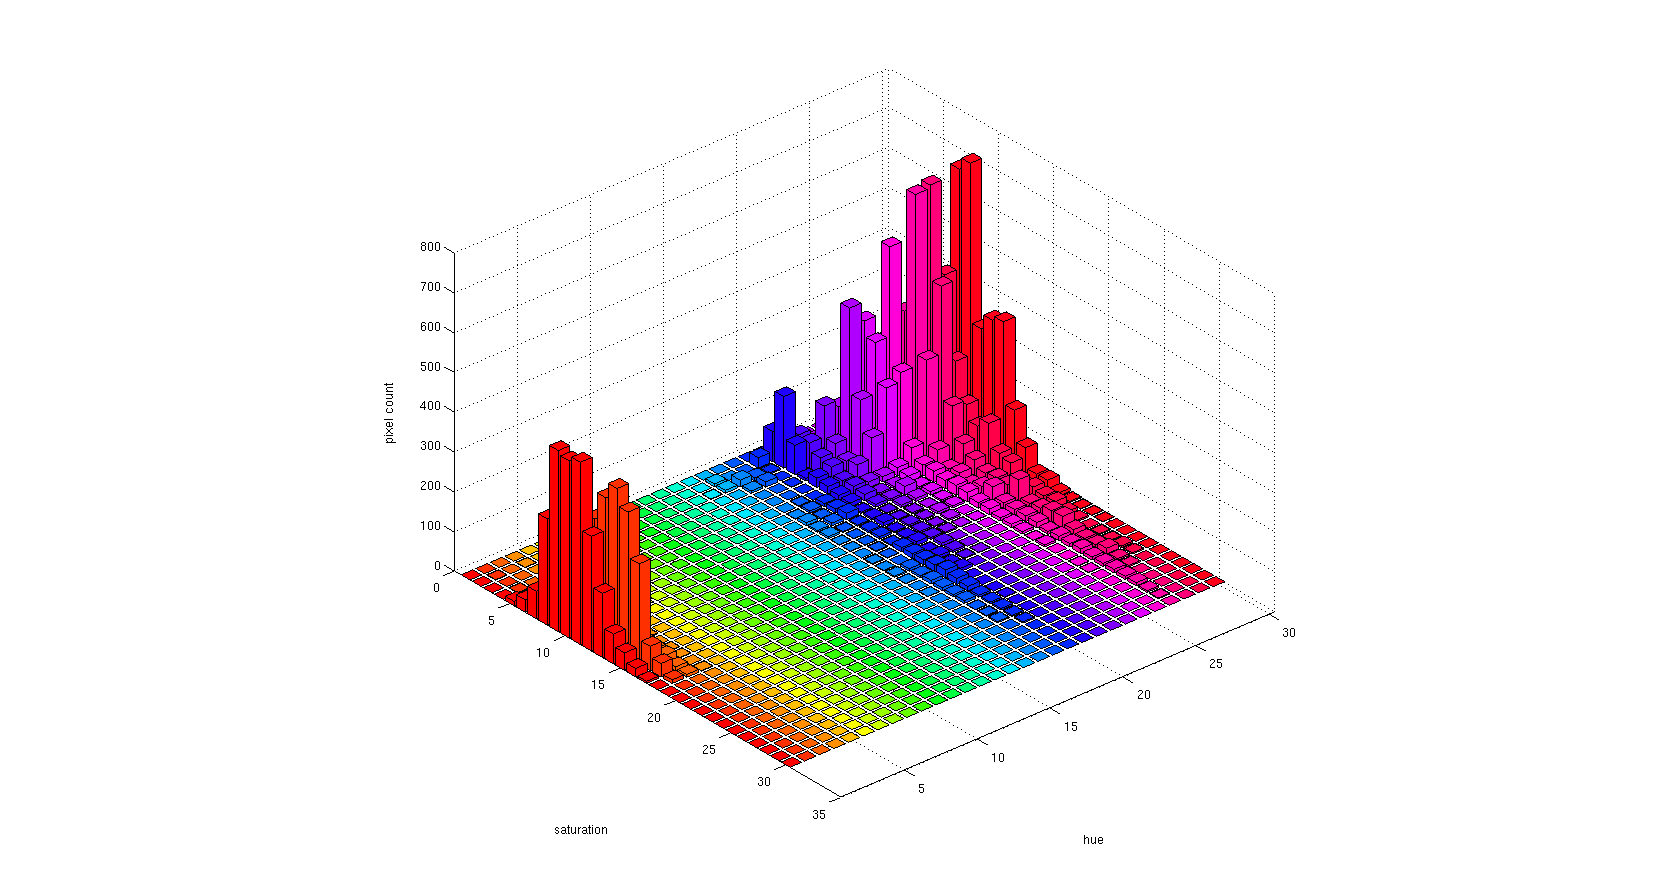
\includegraphics[width=0.3\linewidth]{figures/pipeline/histogram.png}}
\hspace{0.03\linewidth}
\subfloat[Backprojection]{\label{fig:pipe_bp}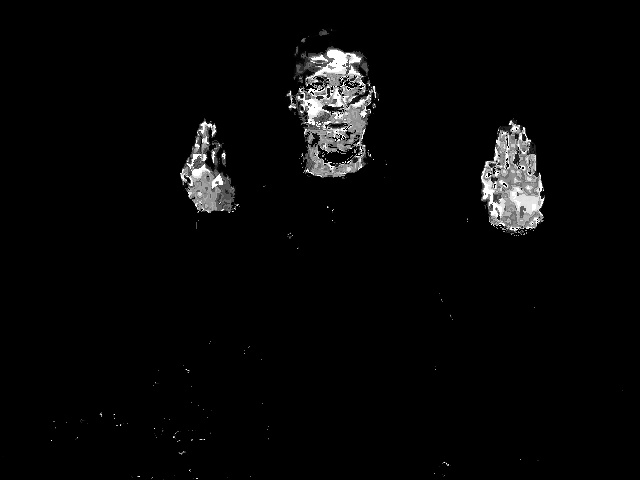
\includegraphics[width=0.3\linewidth]{figures/pipeline/backproject.jpg}}
\hspace{0.03\linewidth}
\subfloat[Gaussian smooth]{\label{fig:pipe_blur}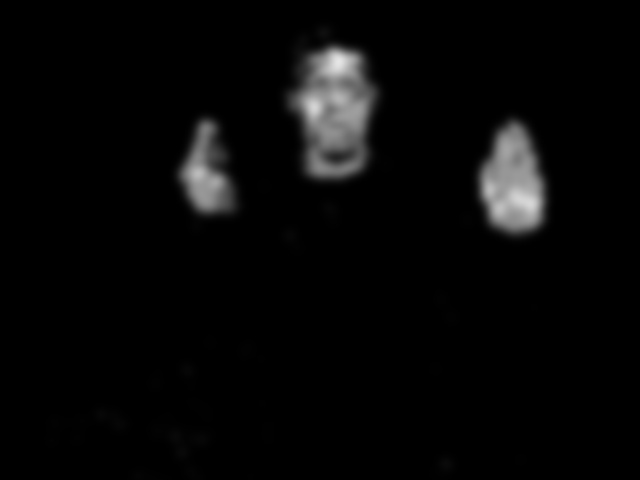
\includegraphics[width=0.3\linewidth]{figures/pipeline/blurred.jpg}}
\hspace{0.03\linewidth}
\subfloat[Thresholded binary image]{\label{fig:pipe_th}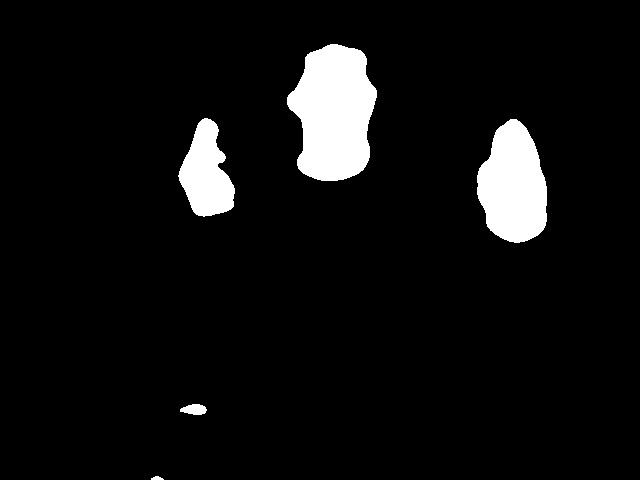
\includegraphics[width=0.3\linewidth]{figures/pipeline/thresholded.jpg}}
\hspace{0.03\linewidth}
\subfloat[Morpholoical close]{\label{fig:pipe_close}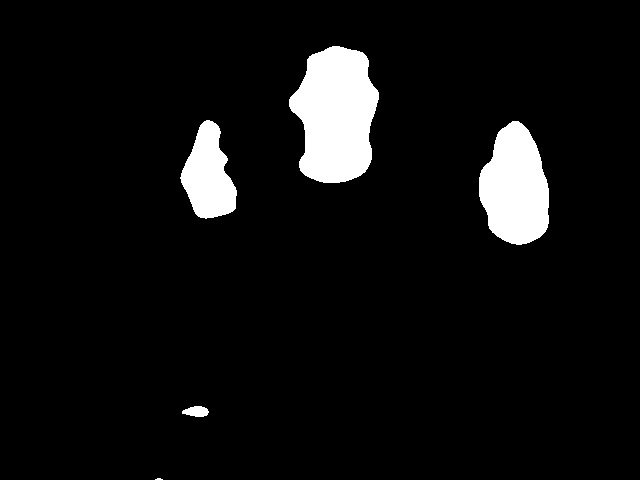
\includegraphics[width=0.3\linewidth]{figures/pipeline/closed.jpg}}
\hspace{0.03\linewidth}
\subfloat[Blob labeling]{\label{fig:pipe_cont}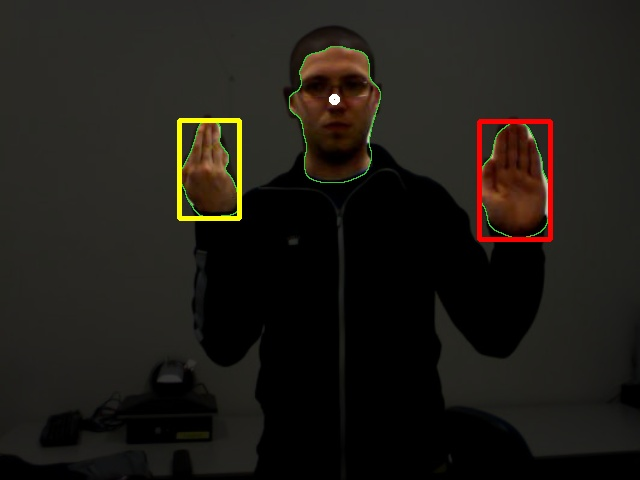
\includegraphics[width=0.3\linewidth]{figures/pipeline/contours.jpg}}
\end{center}
\caption{The hand detection pipeline}
\label{fig:pipeline}
\end{figure}

